%!TEX root = ../template.tex
%%%%%%%%%%%%%%%%%%%%%%%%%%%%%%%%%%%%%%%%%%%%%%%%%%%%%%%%%%%%%%%%%%%
%% chapter1.tex
%% NOVA thesis document file
%%
%% Chapter with introduction
%%%%%%%%%%%%%%%%%%%%%%%%%%%%%%%%%%%%%%%%%%%%%%%%%%%%%%%%%%%%%%%%%%%
\newcommand{\novathesis}{\emph{novathesis}}
\newcommand{\novathesisclass}{\texttt{novathesis.cls}}


%%-------------------------------------------------------------------
%%	1 - Introduction
%%-------------------------------------------------------------------
\chapter{Introduction}
\label{cha:introduction}

%\begin{quotation}
%  \itshape
%  This work is licensed under the Creative Commons Attribution-NonCommercial~4.0 International License.
%  To view a copy of this license, visit \url{http://creativecommons.org/licenses/by-nc/4.0/}.
%\end{quotation}


%%-------------------------------------------------------------------
%%	1.1 - Context
%%-------------------------------------------------------------------
\section{Context} % (fold)
\label{sec:context}

The concept of virtualisation, despite all the recent discussion, isn’t new. In reality, this technology has been around since the 1960s~\cite{Buzen1973}, but not until the development of virtualisation technologies for the x86 architecture~\cite{Agesen2010} and the introduction of \textit{Intel VT}~\cite{Intel2010} and \textit{AMD SVM}~\cite{AMD2010} in the 2000s entered the mainstream as the go-to technology solution for server deployment across many production environments. 

With efficient techniques that take advantage of all available resources, and a lowering price point on hardware, an opportunity for the advance of new application models and a revamp in the supporting infrastructure was generated. 

However, companies realised that the cost to run a fully fledged \textit{data centre} in-house is unreasonable and a cumbersome task. Not only taking into account the cost of the machines, but factoring in the many requirements like the cooling systems that take care of the heat generated by the running machines, physical security to protect the rooms, fire suppressing systems in case of emergency, people to maintain the infrastructure, all added, result in considerable costs on a monthly basis.
Adding to this, the demand for instantaneous access to information and the extensive resources needed to store it does not stop growing.

This fact created an opening for a \gls{IaaS}~\cite{Mell2011} model, outsourcing all the responsibilities of storing the data and providing the needed computation resources from third parties, which are experts in maintaining huge data centres and even provide all this in various geographic regions.

With influential industry players following this trend, supporting more and more types of services and with an increasing number of customers joining this model, new ways to store the growing number of files have emerged. New file systems with a focus on reliability, consistency, performance, scalability, all in a distributed architecture are essential to a broad range of applications presenting a myriad of workloads.



%%-------------------------------------------------------------------
%%	1.2 - Motivation
%%-------------------------------------------------------------------
\section{Motivation} % (fold)
\label{sec:motivation}

Virtualisation is the pillar technology that allowed for the widespread of the IaaS cloud providers in a model of economies of scale. These cloud providers, such as Amazon AWS~\cite{aws_2017}, Microsoft Azure~\cite{azure_2017} and Google Cloud Platform~\cite{gcp_2017}, manage thousands of physical machines all over the globe, with the majority of the infrastructure being multi-tenant oriented. 

The sheer magnitude of those numbers leads to an obvious problem. How to store all this data efficiently? Not only there is the need to store client generated data but also manage all the demands of the infrastructure and the many services offered. One approach taken by these companies was the development of their proprietary storage solutions. For instance, Google uses BigTable distributed storage system \cite{Chang2006}, to store product specific data, and then serve it to users. This system relies on the Google File System underneath to provide a robust solution to store logs and data files, designed to be reliable, scalable and fault tolerance.

One characteristic in particular that stands out and is present in many of today's systems is the use of snapshots with copy-on-write techniques. The adoption of such methods allows for quick copy operations of large data sets but saving resources. At the same time, it provides high-availability with read-only copies of the data always ready to use and allowing applications to continue execution of write operations simultaneously.
All the above-mentioned properties joined with others such as replication and data distribution, to comprise the fundamentals of what is needed to run a highly distributed and scalable file system. For instance, the duplication of records across multiple machines, not only serves as a security net in case of a misfortune event avoiding having a single point of failure but can also be used to maximise availability and take advantage of network bandwidth. 

%Existing file systems address some of these properties by default, however, in most cases, they were designed to be compatible with an increasing diversity of devices that run UNIX-based Operating Systems and need to offer a POSIX API, being more concerned with a local environment. 
%TODO
%\textbf{TO DO - Rephrase sentence above}\\

One of these newer systems that have a significant adoption by the Linux community is the BTRFS~\cite{Rodeh2013}. At the start, this file system already adopts an efficient system of snapshots, and it has as a primary design principle to maintain excellent performance in a comprehensive set of conditions.
The combination of this file system with replication and partitioning techniques opens the way to a solution that serves the needs of an up to date storage system, consequently having the possibility of being easily integrated into an existing platform, serving a vast number of clients and presenting outstanding performance. 



%%-------------------------------------------------------------------
%%	1.3 - Project Presentation
%%-------------------------------------------------------------------
\section{Project Presentation} % (fold)
\label{sec:project_presentation}

This dissertation work is performed in the context of a more comprehensive project with the name \gls{iCBD}~\cite{Lopes2017}, under development at Reditus S.A. in collaboration with DI - FCT/NOVA.
The primary objective is to improve in a known model, the client-based Virtual Desktop Infrastructure, developing an infrastructure to support the execution, in a non-intrusive way, of virtualised desktops in conventional workstations.

%This dissertation work in enveloped in a larger project by the name iCBD, Infrastructure for Client-Based (Virtual) Desktop (Computing), were the objectives pass by the development of a computational infrastructure capable of supporting the execution of virtual desktops in an assortment of devices having as its main characteristic a non-intrusive approach. 

%Taking this into account, there is a clear separation from other solutions previously and currently available, where there is a concern for the target device, without any writing being done to the local disks, preserving all the stored data, and giving the possibility to have other operating systems available for a local boot. To achieve this objective, all the needed components are loaded on-demand at the system startup and as part of the boot.

% section project_presentation (end)


%%-------------------------------------------------------------------
%%	1.3. - Previous Work
%%-------------------------------------------------------------------
\subsection{iCBD Project} % (fold)
\label{sub:icbd_project}


There are some leading-edge aspects of the \acrfull{iCBD} project which sets it apart from other existing solutions such as the adoption of a diskless paradigm with a remote boot, the way virtual machine images are stored in the platform, and the support for a virtualised or native execution on the target workstation, depending on the user's choice.~\cite{P2020}

The Remote boot support is offered by \acrshort{HTTP}, \acrshort{TFTP}, and \acrshort{DHCP} servers, and in turn, the image repository servers manage the storage of the VMs templates and the production of instances based on them.
To address the process of communication between workstations and the platform it is used the HTTP protocol, providing flexibility and efficiency in the communication of the messages.~\cite{P2020,Nuno2016,Eduardo2016}

%\begin{figure}[htbp]
%	\centering
%	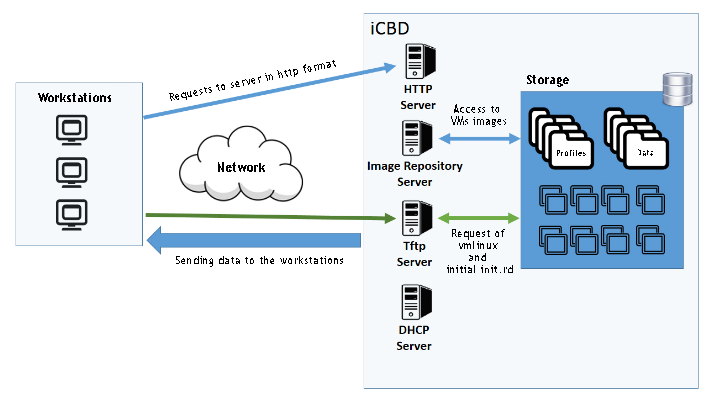
\includegraphics[height=3in]{cap1_icbd}
%	\caption{iCBD architecture. Adapted from \enquote{Linked clones baseados em funcionalidades de snapshot do sistema de ficheiros} by Nuno Alves~\cite{Nuno2016}}
%	\label{fig:icbd}
%\end{figure}

%\newpage

It is also interesting to briefly discuss some of the primary objectives of the project, being:
\begin{itemize}
	%
	\item Offer a work environment and experience of use so close to the traditional one, that there is no disruption for the users when they begin to use this platform.
	%
	\item Enable centralized management of the entire infrastructure including servers in their multiple roles, storage and network devices from a single point.
	%
	\item Complete decoupling between users and workstations in order to promote mobility.
	%
	\item Support the disconnected operation of mobile workstations.
	%
\end{itemize}

With all the above in account, there is a clear separation from other solutions previously and currently available. As far as we know, no other solution is so comprehensive in the use of the resources offered by workstations whether they are PCs, laptops or similar devices.

%This dissertation work is part of a larger project designated iCBD, Infrastructure for Client-Based (virtual) Desktop (computing), under development at Reditus S.A. in collaboration with DI - FCT/NOVA.

%The primary objective is to improve in a known model, the client-based Virtual Desktop Infrastructure, devising an infrastructure to support the execution, in a non-intrusive way, of virtualized desktops in conventional workstations.

% subsection icbd_project (end)


%%-------------------------------------------------------------------
%%	1.3. - Previous Work
%%-------------------------------------------------------------------
\subsection{Previous Work} % (fold)
\label{sub:previous_work}

There have previously been two dissertations involved in this project. That work has centred in the creation of the instances of virtual machines, more specifically in the creation supported by native snapshot mechanisms of the file system where the templates are stored. This way instead of using the hypervisor itself as a method to provision full or thin clones the work is done by the file system snapshot system.

As is happening now, the two theses have followed two different paths in an attempt to determine which file system best suits these objectives. Being that one used a local file system, the BTRFS, and the other followed the object-based storage path, adopting the CephFS.

% subsection previous_work (end)

%%-------------------------------------------------------------------
%%	1.4 - Project Contributions
%%-------------------------------------------------------------------
%\section{Project Framing and Contributions} % (fold)
\section{Problem Stating and Project Contributions}
\label{sec:project_contributions}

This work, as a part of a bigger project and building on previous contributions, has as premise a couple of existing technologies in the file systems field to create a replicated and distributed environment capable of storing large files consisting mainly of \textit{VMs} templates and golden images. This work not only focuses on storage management aspects, as also attends the need of being integrated into a larger infrastructure and coexist with a wide variety of other systems.

%%-------------------------------------------------------------------
%%	3.2. - Replication and Caching - The Problem 
%%-------------------------------------------------------------------
\subsection{Replication and Caching - The Problem}
\label{sec:replication_cache_theproblem}

!!! \textbf{TODO} - Intro!!!


%\subsection{Motivation and Goals}
\paragraph{Motivation and Goals}
\label{par:motivation_goals}

!!! \textbf{TODO} !!!

\textbf{TOPICS :}
\begin{itemize}
	\item The iCBD platform needs to be available and maintain top notch performance in multiple locations while serving a considerable number of clients
	\item Produce a mechanism that allows the replication of data not only for security reasons (backup) but also providing that data closer to the client
	\item With the data near its consumer how to deliver that data to the client? (cache server)
	\item What are the procedures that need to reside near the client (aka why the administration process can be centralised)
\end{itemize}



%\subsubsection{Replication}
\paragraph{Replication}
\label{par:replication_goals}

!!! \textbf{TODO} !!!

\textbf{TOPICS :}
\begin{itemize}
	\item Create a middleware that integrates with the core functionalities of the iCBD platform
	\item Should try to be storage provider agnostic (in this thesis work with BTRFS but easy to integrate with others)
	\item Work with compression algorithms to achieve a lower bandwidth consumption.
	\item Be able to use encrypted and unencrypted communications
	\item Capitalize the snapshotting features of the storage system in order to minimise the volume of data transferred
	\item Provide a simple CLI and API
\end{itemize}



%\subsubsection{Cache Servers}
\paragraph{Cache Servers}
\label{par:caching_goals}

!!! \textbf{TODO} !!!

\textbf{TOPICS :}
\begin{itemize}
	\item Dilute some cost of the infrastructure by having commodity hardware as proximity servers.
	\item Bring the date closer to the final clients
	\item Facilitate a user experience like the OS was installed in a local hard drive
	\item Study the benefits of introducing cache servers in the platform 
\end{itemize}


%\subsection{System Overview}
%\label{sub:system_overview}

%\subsection{Requirements}
%\label{sub:requirements}



%%-------------------------------------------------------------------
%%	1.3. - Main Expected Contributions
%%-------------------------------------------------------------------
\subsection{Main Expected Contributions} % (fold)
\label{sub:main_expected_contributions}

The main expected contributions are: 

\begin{itemize}

  \item The study, develop, and evaluate an implementation of a distributed and replicated BTRFS file system for VM storage.
  \item Implement a server-side caching solution in order to increase availability, improve response time, and enable better management of resources.
  \item Integrate the solutions described above  with the work previously developed and the existing infrastructure
  \item And finally, carry out a series of tests that lead to a meaningful conclusion and that provide help in the design of the remaining platform.

\end{itemize}

A detailed view of the planning can be found in \textbf{Chapter~\ref{sec:work_plan}}.

% subsection main_expected_contributions (end)


%%-------------------------------------------------------------------
%%	1.5 - Document Structure
%%-------------------------------------------------------------------
\section{Document Structure} % (fold)
\label{sec:document_structure}

The remnant document is structured as follows: 

\begin{itemize}

  \item \textit{Chapter~\ref{cha:related_work}}  \textbf{Related Work} - This section presents existing technologies and theoretical approaches which were the target of study, such as, storage systems and several of its features, as well as several intrinsic characteristics of virtualization techniques.

  \item \textit{Chapter 3} \textbf{Proposed Work} - In this chapter, there is a presentation of the work plan for the elaboration of this dissertation. Giving also an overview of the solution to develop on the duration of this thesis.

\end{itemize}

% section document_structure (end)
